\appendix
\chapter{Cavity for frequency stability of spin-sensitive tweezer}%
\label{ch:app_cavity}

A special cavity was built in order to stabilize the spin-sensitive tweezer against its frequency. The outer housing is made of stainless steel and can be evacuated using the flange in the back. The cavity is a \ac{ule} spacer, resting on a copper block, which should absorb most temperature instabilities. The spacer is surrounded by Viton rings, to prevent it from damage against direct contact with the copper block. Not visible are peek spacer between the copper block and steel casing, which isolate both parts from each other. A picture of the cavity is given below, in Figure~\ref{fig:cavity_image}.

\begin{figure}[h!]%
\label{fig:cavity_image}
\centering{%
	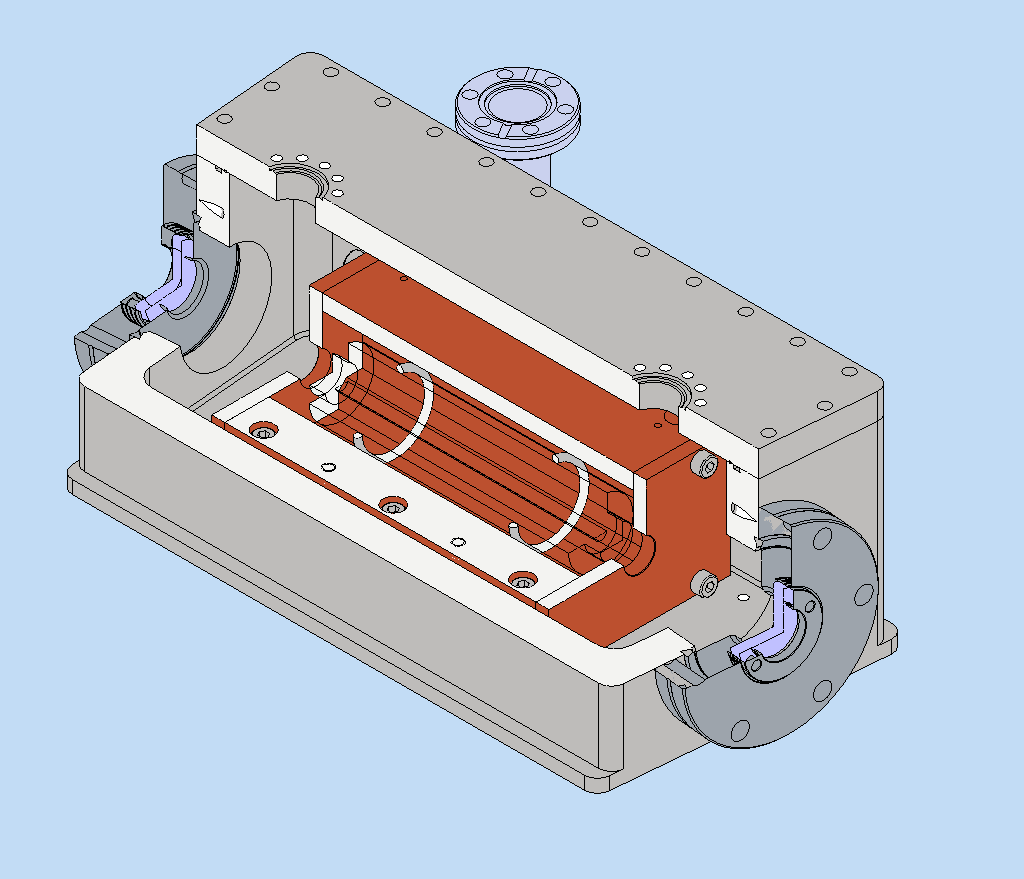
\includegraphics[width=\textwidth]{figures/cavity_image.png}
	\caption{The cavity used for frequency locking the spins-sensitive tweezer.}
}
\end{figure}
